\documentclass[12pt]{letter}

%%%%%%%%%%%%%%%%%% PACKAGES %%%%%%%%%%%%%%%%%%%%%%%%%%
\usepackage[french]{babel}
\usepackage{amssymb}
\usepackage{amsmath}
\usepackage{a4wide}
\usepackage{stmaryrd}
\usepackage{amscd}
\usepackage{enumerate}
\usepackage{graphicx} 
\usepackage{amsfonts}
\usepackage[utf8]{inputenc}  
\usepackage{tikz}
\usepackage{multirow}
\usepackage{array}
\usepackage{relsize}
\usepackage{listings}
\definecolor{dkgreen}{rgb}{0,0.6,0}
\definecolor{gray}{rgb}{0.5,0.5,0.5}
\definecolor{mauve}{rgb}{0.58,0,0.82}
%%%%%%%%%%%%%%%%%%%%%%%%%%%%%%%%%%%%%%%%%%%%%%%%%%
\lstset{ %
  language=python,                % the language of the code
  framerule=0pt,
  basicstyle=\relsize{-2}\ttfamily,  % the size of the fonts that are used for the code
  %backgroundcolor=\color{black!10},  % choose the background color. You must add \usepackage{color}
  showspaces=false,               % show spaces adding particular underscores
  showstringspaces=false,         % underline spaces within strings
  showtabs=false,                 % show tabs within strings adding particular underscores
  %frame=single,                   % adds a frame around the code
  rulecolor=\color{black},        % if not set, the frame-color may be changed on line-breaks within not-black text (e.g. commens (green here))
  breakatwhitespace=false,        % sets if automatic breaks should only happen at whitespace
  keywordstyle=\color{blue},      % keyword style
  commentstyle=\color{dkgreen},   % comment style
  stringstyle=\color{mauve}  
}

\begin{document}

%%%%%%%%%%%%%%%%% TITRE %%%%%%%%%%%%%%%%%%%%%%%%%%
\begin{center}
{\Large Exercices  }
\end{center}

%%%%%%%%%%%%%%%%%%%%%%%%%%%%%%%%%%%%%%%%%%%%%%%%%%%%
\textbf{Date de naissance}
\begin{enumerate}
   \item faire tourner le code fourni en exemple \texttt{date.py}
\end{enumerate}

\textbf{Animation graphique}

 Le but de cet exercice est de vous montrer comment la programmation peut intervenir dans une animation graphique simple ``d'images de synthèse''.
 On considérera dans ce cadre, juste le coté géométrique de l'animation. Dans le squelette fourni en TP, on a déjà un début d'animation: 
 une sphère qui suit une trajectoire rectiligne. 
 Pour situer la sphère aux coordonnées $(x,y,z)$ dans le repère choisi, on utilisera l'instruction \texttt{sphereActor.SetPosition(x,y,z)}
 Dans l'exemple donné, on fait varier la coordonnée $y$ de la sphère. 

 \begin{enumerate} 
 
    \item Faire tourner le programme. Pour régler la position de la caméra, utiliser
    la souris et presser \texttt{e} pour lancer l'animation. Enlever le commentaire devant la ligne
    \texttt{ren1.GetActiveCamera().Azimuth( 0.2 )} pour tourner autour de la scène durant l'animation
    \item essayer de programmer un rebond quand on détecte des coordonnées $y$ négatives, en utilisant le schéma suivant 
   \begin{center}
     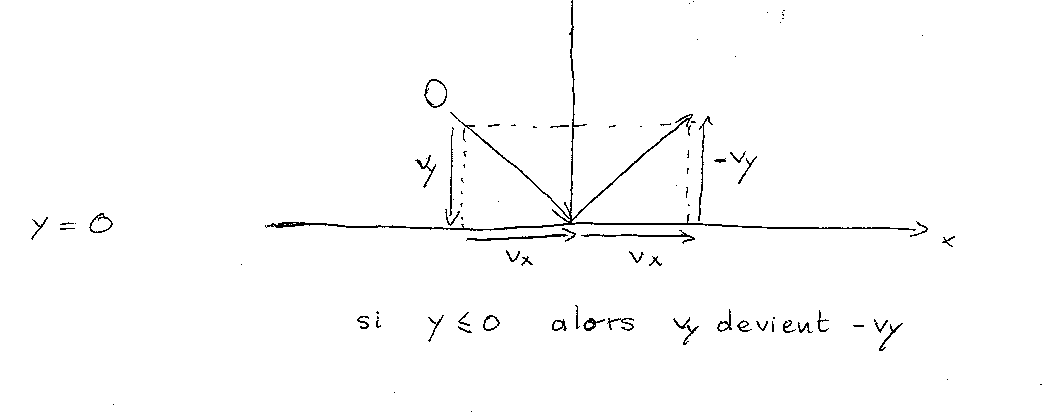
\includegraphics[width=0.8\linewidth]{rebond.pdf}
   \end{center}
   On pourra utiliser un \texttt{if} dans la boucle en temps. Bien penser à remettre $y$ à zéro pour rebondir
   \item programmer un rebond quand $y \geqslant H$
   \item on introduit de la même façon les composantes $v_x$ et $v_z$ de la vitesse. Programmer les tests de bords ($x <0$, $z < 0$ et $x > L$, $z > P$)
   \item on peut ajouter du frein $vx *= -\alpha$ où $\alpha < 1$ pour ralentir la balle quand elle rebondit.
   \item voila, on a notre animation graphique. En allant regarder la documentation de VTK(\texttt{ www.vtk.org}), éditer le fichier \texttt{cree\_scene.py}
   pour modifier les paramètres de l'animation (forme de la boule, couleurs de fond, etc...)
    
  \end{enumerate}
\end{document}


